%! TeX program = lualatex
%! TeX root = main.tex

\def\basedir{/home/theammir/labs/asd/9/res}
\input{/home/theammir/labs/asd/template/template.tex}

\usepackage{graphicx}
\usepackage[hypcap=false]{caption}

\begin{document}
\thetitlepage{10}{ІМ-42}{Туров Андрій Володимирович}{28}

\taskdesc%
\begin{enumerate}
  \item Представити напрямлений та ненапрямлений графи iз заданими параметрами так само, як у лабораторнiй роботi №3.\par
    \emph{Вiдмiннiсть:} коефiцiєнт $k = 1.0 - n_3 * 0.01 - n_4 * 0.01 - 0.3$.
  \item Обчислити:
    \begin{enumerate}
      \item степенi вершин напрямленого i ненапрямленого графiв;
      \item напiвстепенi виходу та заходу напрямленого графа;
      \item чи є граф однорiдним (регулярним), i якщо так, вказати степiнь однорiдностi графа;
      \item перелiк висячих та iзольованих вершин.
    \end{enumerate}
  \item Змiнити матрицю $A_{dir}$, коефiцiєнт $k = 1.0 * n_3 * 0.005 * n_4 * 0.005 * 0.27$.
  \item Для нового орграфа обчислити:
  \begin{enumerate}
    \item пiвстепенi вершин;
    \item всi шляхи довжини 2 i 3;
    \item матрицю досяжностi;
    \item матрицю сильної зв’язностi;
    \item перелiк компонент сильної зв’язностi;
    \item граф конденсацiї.
  \end{enumerate}
\end{enumerate}

\taskspec%
$\overline{n_1 n_2 n_3 n_4} = 4228$;\\
Кількість вершин --- $10 + n_3 = 12$.\\
Розміщення вершин --- прямокутником з вершиною в центрі.

\codetext{rust}

\section{Матриці суміжності}

\begin{minipage}[t]{0.4\linewidth}
  \begin{framed}
    \noindent%
    Для напрямленого графа:\\\\
    \raggedright\footnotesize\texttt{%
      0 0 1 0 0 0 0 0 0 0 1 0\\
      0 0 0 1 0 0 0 0 0 0 0 1\\
      0 0 0 0 0 1 0 0 0 0 0 0\\
      0 0 1 1 0 1 0 1 0 0 0 0\\
      0 0 0 0 0 0 1 0 0 0 1 0\\
      0 0 0 0 0 1 0 1 0 0 0 0\\
      0 0 0 0 0 0 0 0 0 0 1 0\\
      0 0 0 0 0 0 0 0 0 0 0 0\\
      0 0 0 0 0 1 0 0 0 0 1 0\\
      1 0 1 0 0 0 0 0 0 0 0 0\\
      0 0 0 0 0 1 0 0 0 0 1 0\\
      0 0 0 1 0 1 0 0 1 0 0 0\\
    }
  \end{framed}
\end{minipage}
\hfill
\begin{minipage}[t]{0.4\linewidth}
  \begin{framed}
    \noindent%
    Для ненапрямленого графа:\\\\
    \raggedright\footnotesize\texttt{%
      0 1 1 0 0 0 1 0 0 0 1 0\\
      1 0 0 1 0 0 0 1 0 0 1 1\\
      1 0 1 0 0 1 1 0 0 0 0 0\\
      0 1 0 1 0 1 0 1 1 1 0 1\\
      0 0 0 0 0 0 1 0 0 0 1 0\\
      0 0 1 1 0 1 0 1 0 1 0 0\\
      1 0 1 0 1 0 0 0 0 0 1 0\\
      0 1 0 1 0 1 0 0 0 1 0 0\\
      0 0 0 1 0 0 0 0 0 0 1 0\\
      0 0 0 1 0 1 0 1 0 0 0 0\\
      1 1 0 0 1 0 1 0 1 0 1 1\\
      0 1 0 1 0 0 0 0 0 0 1 1\\
    }
  \end{framed}
\end{minipage}
\hfill

\section{Характеристика вершин}
\begin{framed}
  \noindent%
  Для напрямленого графа:\\\\
  \raggedright\footnotesize\texttt{%
    Vertex semi-degrees (IN):  1 0 3 3 0 6 1 2 1 0 5 1\\
    Vertex semi-degrees (OUT): 2 2 1 4 2 2 1 0 2 2 2 3\\
    Vertex degrees:            3 2 4 7 2 8 2 2 3 2 7 4\\
    Is regular: false\\
    Isolated vertices:\\
    Pendant vertices:\\
  }
\end{framed}
\begin{framed}
  \noindent%
  Для ненапрямленого графа:\\\\
  \raggedright\footnotesize\texttt{%
    Vertex degrees:            4 4 4 8 4 8 4 4 2 0 10 2\\
    Is regular: false\\
    Isolated vertices:         10\\
    Pendant vertices:\\
  }
\end{framed}
\hfill

\section{Модифікований граф}
\begin{minipage}[t]{0.45\linewidth}
  \begin{framed}
    \noindent%
    Матриця суміжності:\\\\
    \raggedright\footnotesize\texttt{%
        0 1 1 1 0 0 1 0 0 0 1 0\\
        0 0 0 1 0 0 0 1 0 0 1 1\\
        0 0 1 0 0 1 1 0 0 0 0 0\\
        0 0 1 1 0 1 0 1 1 1 0 1\\
        0 0 0 0 0 0 1 0 0 0 1 0\\
        0 0 0 0 0 1 0 1 0 1 0 0\\
        0 0 1 0 0 0 0 0 0 0 1 0\\
        0 0 1 0 0 0 0 0 0 1 0 0\\
        0 1 0 0 0 1 0 0 1 0 1 1\\
        1 0 1 0 0 0 1 0 0 0 0 0\\
        0 0 0 0 0 1 0 0 0 0 1 1\\
        1 0 1 1 0 1 1 0 1 1 0 1\\
    }
  \end{framed}
\end{minipage}
\begin{minipage}[t]{0.45\linewidth}
  \begin{framed}
    \noindent%
    Напівстепені вершин:\\
    \raggedright\footnotesize\texttt{%
      vertex semi-degrees (in):  2 2 7 4 0 6 5 3 3 4 6 5\\
      vertex semi-degrees (out): 5 4 3 7 2 3 2 2 5 3 3 8\\
    }
  \end{framed}
\end{minipage}
\hfill
\begin{framed}
  \noindent%
  Усі шляхи довжини 2:\\
  \raggedright\footnotesize\texttt{%
    Paths of 2: 1->3->3 1->4->3 1->7->3 1->2->4 1->4->4 1->3->6 1->4->6 1->11->6 1->3->7 1->2->8 1->4->8 1->4->9 1->4->10 1->2->11 1->7->11 1->11->11 1->2->12 1->4->12 1->11->12 2->12->1 2->4->3 2->8->3 2->12->3 2->4->4 2->12->4 2->4->6 2->11->6 2->12->6 2->12->7 2->4->8 2->4->9 2->12->9 2->4->10 2->8->10 2->12->10 2->11->11 2->4->12 2->11->12 2->12->12 3->3->3 3->7->3 3->3->6 3->6->6 3->3->7 3->6->8 3->6->10 3->7->11 4->10->1 4->12->1 4->9->2 4->3->3 4->4->3 4->8->3 4->10->3 4->12->3 4->4->4 4->12->4 4->3->6 4->4->6 4->6->6 4->9->6 4->12->6 4->3->7 4->10->7 4->12->7 4->4->8 4->6->8 4->4->9 4->9->9 4->12->9 4->4->10 4->6->10 4->8->10 4->12->10 4->9->11 4->4->12 4->9->12 4->12->12 5->7->3 5->11->6 5->7->11 5->11->11 5->11->12 6->10->1 6->8->3 6->10->3 6->6->6 6->10->7 6->6->8 6->6->10 6->8->10 7->3->3 7->3->6 7->11->6 7->3->7 7->11->11 7->11->12 8->10->1 8->3->3 8->10->3 8->3->6 8->3->7 8->10->7 9->12->1 9->9->2 9->12->3 9->2->4 9->12->4 9->6->6 9->9->6 9->11->6 9->12->6 9->12->7 9->2->8 9->6->8 9->9->9 9->12->9 9->6->10 9->12->10 9->2->11 9->9->11 9->11->11 9->2->12 9->9->12 9->11->12 9->12->12 10->1->2 10->1->3 10->3->3 10->7->3 10->1->4 10->3->6 10->1->7 10->3->7 10->1->11 10->7->11 11->12->1 11->12->3 11->12->4 11->6->6 11->11->6 11->12->6 11->12->7 11->6->8 11->12->9 11->6->10 11->12->10 11->11->11 11->11->12 11->12->12 12->10->1 12->12->1 12->1->2 12->9->2 12->1->3 12->3->3 12->4->3 12->7->3 12->10->3 12->12->3 12->1->4 12->4->4 12->12->4 12->3->6 12->4->6 12->6->6 12->9->6 12->12->6 12->1->7 12->3->7 12->10->7 12->12->7 12->4->8 12->6->8 12->4->9 12->9->9 12->12->9 12->4->10 12->6->10 12->12->10 12->1->11 12->7->11 12->9->11 12->4->12 12->9->12 12->12->12 
  }
\end{framed}
\begin{framed}
  \noindent%
  Усі шляхи довжини 3:\\
  \raggedright\footnotesize\texttt{%
    Paths of 3: 1->2->12->1 1->4->10->1 1->4->12->1 1->11->12->1 1->4->9->2 1->2->4->3 1->2->8->3 1->2->12->3 1->3->3->3 1->3->7->3 1->4->3->3 1->4->4->3 1->4->8->3 1->4->10->3 1->4->12->3 1->7->3->3 1->11->12->3 1->2->4->4 1->2->12->4 1->4->4->4 1->4->12->4 1->11->12->4 1->2->4->6 1->2->11->6 1->2->12->6 1->3->3->6 1->3->6->6 1->4->3->6 1->4->4->6 1->4->6->6 1->4->9->6 1->4->12->6 1->7->3->6 1->7->11->6 1->11->6->6 1->11->11->6 1->11->12->6 1->2->12->7 1->3->3->7 1->4->3->7 1->4->10->7 1->4->12->7 1->7->3->7 1->11->12->7 1->2->4->8 1->3->6->8 1->4->4->8 1->4->6->8 1->11->6->8 1->2->4->9 1->2->12->9 1->4->4->9 1->4->9->9 1->4->12->9 1->11->12->9 1->2->4->10 1->2->8->10 1->2->12->10 1->3->6->10 1->4->4->10 1->4->6->10 1->4->8->10 1->4->12->10 1->11->6->10 1->11->12->10 1->2->11->11 1->3->7->11 1->4->9->11 1->7->11->11 1->11->11->11 1->2->4->12 1->2->11->12 1->2->12->12 1->4->4->12 1->4->9->12 1->4->12->12 1->7->11->12 1->11->11->12 1->11->12->12 2->4->10->1 2->4->12->1 2->8->10->1 2->11->12->1 2->12->10->1 2->12->12->1 2->4->9->2 2->12->1->2 2->12->9->2 2->4->3->3 2->4->4->3 2->4->8->3 2->4->10->3 2->4->12->3 2->8->3->3 2->8->10->3 2->11->12->3 2->12->1->3 2->12->3->3 2->12->4->3 2->12->7->3 2->12->10->3 2->12->12->3 2->4->4->4 2->4->12->4 2->11->12->4 2->12->1->4 2->12->4->4 2->12->12->4 2->4->3->6 2->4->4->6 2->4->6->6 2->4->9->6 2->4->12->6 2->8->3->6 2->11->6->6 2->11->11->6 2->11->12->6 2->12->3->6 2->12->4->6 2->12->6->6 2->12->9->6 2->12->12->6 2->4->3->7 2->4->10->7 2->4->12->7 2->8->3->7 2-h8->10->7 2->11->12->7 2->12->1->7 2->12->3->7 2->12->10->7 2->12->12->7 2->4->4->8 2->4->6->8 2->11->6->8 2->12->4->8 2->12->6->8 2->4->4->9 2->4->9->9 2->4->12->9 2->11->12->9 2->12->4->9 2->12->9->9 2->12->12->9 2->4->4->10 2->4->6->10 2->4->8->10 2->4->12->10 2->11->6->10 2->11->12->10 2->12->4->10 2->12->6->10 2->12->12->10 2->4->9->11 2->11->11->11 2->12->1->11 2->12->7->11 2->12->9->11 2->4->4->12 2->4->9->12 2->4->12->12 2->11->11->12 2->11->12->12 2->12->4->12 2->12->9->12 2->12->12->12 3->6->10->1 3->3->3->3 3->3->7->3 3->6->8->3 3->6->10->3 3->7->3->3 3->3->3->6 3->3->6->6 3->6->6->6 3->7->3->6 3->7->11->6 3->3->3->7 3->6->10->7 3->7->3->7 3->3->6->8 3->6->6->8 3->3->6->10 3->6->6->10 3->6->8->10 3->3->7->11 3->7->11->11 3->7->11->12 4->4->10->1 4->4->12->1 4->6->10->1 4->8->10->1 4->9->12->1 4->12->10->1 4->12->12->1 4->4->9->2 4->9->9->2 4->10->1->2 4->12->1->2 4->12->9->2 4->3->3->3 4->3->7->3 4->4->3->3 4->4->4->3 4->4->8->3 4->4->10->3 4->4->12->3 4->6->8->3 4->6->10->3 4->8->3->3 4->8->10->3 4->9->12->3 4->10->1->3 4->10->3->3 4->10->7->3 4->12->1->3 4->12->3->3 4->12->4->3 4->12->7->3 4->12->10->3 4->12->12->3 4->4->4->4 4->4->12->4 4->9->2->4 4->9->12->4 4->10->1->4 4->12->1->4 4->12->4->4 4->12->12->4 4->3->3->6 4->3->6->6 4->4->3->6 4->4->4->6 4->4->6->6 4->4->9->6 4->4->12->6 4->6->6->6 4->8->3->6 4->9->6->6 4->9->9->6 4->9->11->6 4->9->12->6 4->10->3->6 4->12->3->6 4->12->4->6 4->12->6->6 4->12->9->6 4->12->12->6 4->3->3->7 4->4->3->7 4->4->10->7 4->4->12->7 4->6->10->7 4->8->3->7 4->8->10->7 4->9->12->7 4->10->1->7 4->10->3->7 4->12->1->7 4->12->3->7 4->12->10->7 4->12->12->7 4->3->6->8 4->4->4->8 4->4->6->8 4->6->6->8 4->9->2->8 4->9->6->8 4->12->4->8 4->12->6->8 4->4->4->9 4->4->9->9 4->4->12->9 4->9->9->9 4->9->12->9 4->12->4->9 4->12->9->9 4->12->12->9 4->3->6->10 4->4->4->10 4->4->6->10 4->4->8->10 4->4->12->10 4->6->6->10 4->6->8->10 4->9->6->10 4->9->12->10 4->12->4->10 4->12->6->10 4->12->12->10 4->3->7->11 4->4->9->11 4->9->2->11 4->9->9->11 4->9->11->11 4->10->1->11 4->10->7->11 4->12->1->11 4->12->7->11 4->12->9->11 4->4->4->12 4->4->9->12 4->4->12->12 4->9->2->12 4->9->9->12 4->9->11->12 4->9->12->12 4->12->4->12 4->12->9->12 4->12->12->12 5->11->12->1 5->7->3->3 5->11->12->3 5->11->12->4 5->7->3->6 5->7->11->6 5->11->6->6 5->11->11->6 5->11->12->6 5->7->3->7 5->11->12->7 5->11->6->8 5->11->12->9 5->11->6->10 5->11->12->10 5->7->11->11 5->11->11->11 5->7->11->12 5->11->11->12 5->11->12->12 6->6->10->1 6->8->10->1 6->10->1->2 6->6->8->3 6->6->10->3 6->8->3->3 6->8->10->3 6->10->1->3 6->10->3->3 6->10->7->3 6->10->1->4 6->6->6->6 6->8->3->6 6->10->3->6 6->6->10->7 6->8->3->7 6->8->10->7 6->10->1->7 6->10->3->7 6->6->6->8 6->6->6->10 6->6->8->10 6->10->1->11 6->10->7->11 7->11->12->1 7->3->3->3 7->3->7->3 7->11->12->3 7->11->12->4 7->3->3->6 7->3->6->6 7->11->6->6 7->11->11->6 7->11->12->6 7->3->3->7 7->11->12->7 7->3->6->8 7->11->6->8 7->11->12->9 7->3->6->10 7->11->6->10 7->11->12->10 7->3->7->11 7->11->11->11 7->11->11->12 7->11->12->12 8->10->1->2 8->3->3->3 8->3->7->3 8->10->1->3 8->10->3->3 8->10->7->3 8->10->1->4 8->3->3->6 8->3->6->6 8->10->3->6 8->3->3->7 8->10->1->7 8->10->3->7 8->3->6->8 8->3->6->10 8->3->7->11 8->10->1->11 8->10->7->11 9->2->12->1 9->6->10->1 9->9->12->1 9->11->12->1 9->12->10->1 9->12->12->1 9->9->9->2 9->12->1->2 9->12->9->2 9->2->4->3 9->2->8->3 9->2->12->3 9->6->8->3 9->6->10->3 9->9->12->3 9->11->12->3 9->12->1->3 9->12->3->3 9->12->4->3 9->12->7->3 9->12->10->3 9->12->12->3 9->2->4->4 9->2->12->4 9->9->2->4 9->9->12->4 9->11->12->4 9->12->1->4 9->12->4->4 9->12->12->4 9->2->4->6 9->2->11->6 9->2->12->6 9->6->6->6 9->9->6->6 9->9->9->6 9->9->11->6 9->9->12->6 9->11->6->6 9->11->11->6 9->11->12->6 9->12->3->6 9->12->4->6 9->12->6->6 9->12->9->6 9->12->12->6 9->2->12->7 9->6->10->7 9->9->12->7 9->11->12->7 9->12->1->7 9->12->3->7 9->12->10->7 9->12->12->7 9->2->4->8 9->6->6->8 9->9->2->8 9->9->6->8 9->11->6->8 9->12->4->8 9->12->6->8 9->2->4->9 9->2->12->9 9->9->9->9 9->9->12->9 9->11->12->9 9->12->4->9 9->12->9->9 9->12->12->9 9->2->4->10 9->2->8->10 9->2->12->10 9->6->6->10 9->6->8->10 9->9->6->10 9->9->12->10 9->11->6->10 9->11->12->10 9->12->4->10 9->12->6->10 9->12->12->10 9->2->11->11 9->9->2->11 9->9->9->11 9->9->11->11 9->11->11->11 9->12->1->11 9->12->7->11 9->12->9->11 9->2->4->12 9->2->11->12 9->2->12->12 9->9->2->12 9->9->9->12 9->9->11->12 9->9->12->12 9->11->11->12 9->11->12->12 9->12->4->12 9->12->9->12 9->12->12->12 10->1->3->3 10->1->4->3 10->1->7->3 10->3->3->3 10->3->7->3 10->7->3->3 10->1->2->4 10->1->4->4 10->1->3->6 10->1->4->6 10->1->11->6 10->3->3->6 10->3->6->6 10->7->3->6 10->7->11->6 10->1->3->7 10->3->3->7 10->7->3->7 10->1->2->8 10->1->4->8 10->3->6->8 10->1->4->9 10->1->4->10 10->3->6->10 10->1->2->11 10->1->7->11 10->1->11->11 10->3->7->11 10->7->11->11 10->1->2->12 10->1->4->12 10->1->11->12 10->7->11->12 11->6->10->1 11->11->12->1 11->12->10->1 11->12->12->1 11->12->1->2 11->12->9->2 11->6->8->3 11->6->10->3 11->11->12->3 11->12->1->3 11->12->3->3 11->12->4->3 11->12->7->3 11->12->10->3 11->12->12->3 11->11->12->4 11->12->1->4 11->12->4->4 11->12->12->4 11->6->6->6 11->11->6->6 11->11->11->6 11->11->12->6 11->12->3->6 11->12->4->6 11->12->6->6 11->12->9->6 11->12->12->6 11->6->10->7 11->11->12->7 11->12->1->7 11->12->3->7 11->12->10->7 11->12->12->7 11->6->6->8 11->11->6->8 11->12->4->8 11->12->6->8 11->11->12->9 11->12->4->9 11->12->9->9 11->12->12->9 11->6->6->10 11->6->8->10 11->11->6->10 11->11->12->10 11->12->4->10 11->12->6->10 11->12->12->10 11->11->11->11 11->12->1->11 11->12->7->11 11->12->9->11 11->11->11->12 11->11->12->12 11->12->4->12 11->12->9->12 11->12->12->12 12->4->10->1 12->4->12->1 12->6->10->1 12->9->12->1 12->12->10->1 12->12->12->1 12->4->9->2 12->9->9->2 12->10->1->2 12->12->1->2 12->12->9->2 12->1->3->3 12->1->4->3 12->1->7->3 12->3->3->3 12->3->7->3 12->4->3->3 12->4->4->3 12->4->8->3 12->4->10->3 12->4->12->3 12->6->8->3 12->6->10->3 12->7->3->3 12->9->12->3 12->10->1->3 12->10->3->3 12->10->7->3 12->12->1->3 12->12->3->3 12->12->4->3 12->12->7->3 12->12->10->3 12->12->12->3 12->1->2->4 12->1->4->4 12->4->4->4 12->4->12->4 12->9->2->4 12->9->12->4 12->10->1->4 12->12->1->4 12->12->4->4 12->12->12->4 12->1->3->6 12->1->4->6 12->1->11->6 12->3->3->6 12->3->6->6 12->4->3->6 12->4->4->6 12->4->6->6 12->4->9->6 12->4->12->6 12->6->6->6 12->7->3->6 12->7->11->6 12->9->6->6 12->9->9->6 12->9->11->6 12->9->12->6 12->10->3->6 12->12->3->6 12->12->4->6 12->12->6->6 12->12->9->6 12->12->12->6 12->1->3->7 12->3->3->7 12->4->3->7 12->4->10->7 12->4->12->7 12->6->10->7 12->7->3->7 12->9->12->7 12->10->1->7 12->10->3->7 12->12->1->7 12->12->3->7 12->12->10->7 12->12->12->7 12->1->2->8 12->1->4->8 12->3->6->8 12->4->4->8 12->4->6->8 12->6->6->8 12->9->2->8 12->9->6->8 12->12->4->8 12->12->6->8 12->1->4->9 12->4->4->9 12->4->9->9 12->4->12->9 12->9->9->9 12->9->12->9 12->12->4->9 12->12->9->9 12->12->12->9 12->1->4->10 12->3->6->10 12->4->4->10 12->4->6->10 12->4->8->10 12->4->12->10 12->6->6->10 12->6->8->10 12->9->6->10 12->9->12->10 12->12->4->10 12->12->6->10 12->12->12->10 12->1->2->11 12->1->7->11 12->1->11->11 12->3->7->11 12->4->9->11 12->7->11->11 12->9->2->11 12->9->9->11 12->9->11->11 12->10->1->11 12->10->7->11 12->12->1->11 12->12->7->11 12->12->9->11 12->1->2->12 12->1->4->12 12->1->11->12 12->4->4->12 12->4->9->12 12->4->12->12 12->7->11->12 12->9->2->12 12->9->9->12 12->9->11->12 12->9->12->12 12->12->4->12 12->12->9->12 12->12->12->12
  }
  \vspace*{0pt}
\end{framed}

\noindent
\begin{minipage}[t]{0.45\linewidth}
  \begin{framed}
    \noindent%
    Матриця досяжності:\\
    \raggedright\footnotesize\texttt{%
      1 1 1 1 0 1 1 1 1 1 1 1\\
      1 1 1 1 0 1 1 1 1 1 1 1\\
      1 1 1 1 0 1 1 1 1 1 1 1\\
      1 1 1 1 0 1 1 1 1 1 1 1\\
      1 1 1 1 1 1 1 1 1 1 1 1\\
      1 1 1 1 0 1 1 1 1 1 1 1\\
      1 1 1 1 0 1 1 1 1 1 1 1\\
      1 1 1 1 0 1 1 1 1 1 1 1\\
      1 1 1 1 0 1 1 1 1 1 1 1\\
      1 1 1 1 0 1 1 1 1 1 1 1\\
      1 1 1 1 0 1 1 1 1 1 1 1\\
      1 1 1 1 0 1 1 1 1 1 1 1\\
    }
  \end{framed}
\end{minipage}
\hfill
\begin{minipage}[t]{0.45\linewidth}
  \begin{framed}
    \noindent%
    Матриця сильної зв'язаності\\
    \raggedright\footnotesize\texttt{%
      1 1 1 1 0 1 1 1 1 1 1 1\\
      1 1 1 1 0 1 1 1 1 1 1 1\\
      1 1 1 1 0 1 1 1 1 1 1 1\\
      1 1 1 1 0 1 1 1 1 1 1 1\\
      0 0 0 0 1 0 0 0 0 0 0 0\\
      1 1 1 1 0 1 1 1 1 1 1 1\\
      1 1 1 1 0 1 1 1 1 1 1 1\\
      1 1 1 1 0 1 1 1 1 1 1 1\\
      1 1 1 1 0 1 1 1 1 1 1 1\\
      1 1 1 1 0 1 1 1 1 1 1 1\\
      1 1 1 1 0 1 1 1 1 1 1 1\\
      1 1 1 1 0 1 1 1 1 1 1 1\\
    }
  \end{framed}
\end{minipage}

\begin{framed}
  \noindent%
  Компоненти сильної зв'язаності\\
  \raggedright\footnotesize\texttt{%
    [[1, 2, 3, 4, 6, 7, 8, 9, 10, 11, 12], [5]]\\
  }
  \normalsize{
    Конденсована матриця суміжності:\\
  }
  \raggedright\footnotesize\texttt{%
    0 0\\
    1 0\\
  }
\end{framed}

\section{Зображення}

\begin{figure}[ht!]
  \center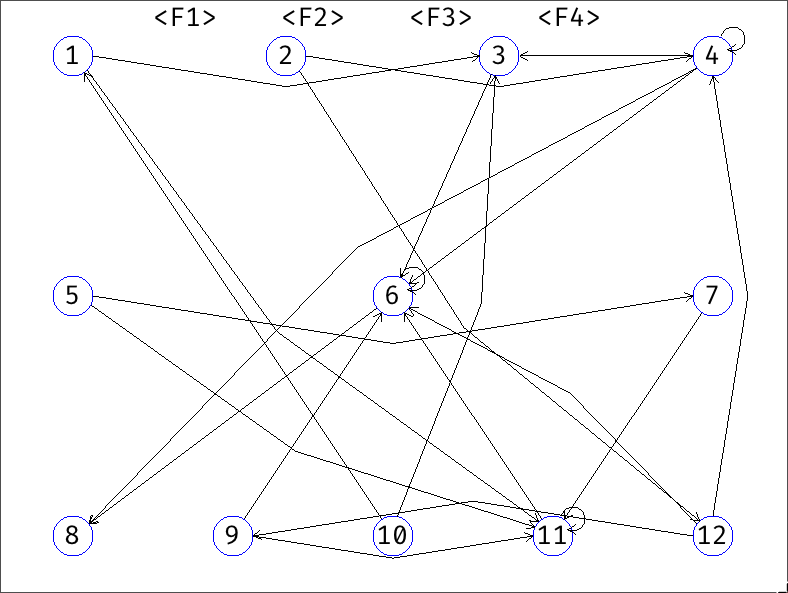
\includegraphics[width=0.5\linewidth]{directed.png}
  \caption{Напрямлений граф}
\end{figure}
\begin{figure}[ht!]
  \center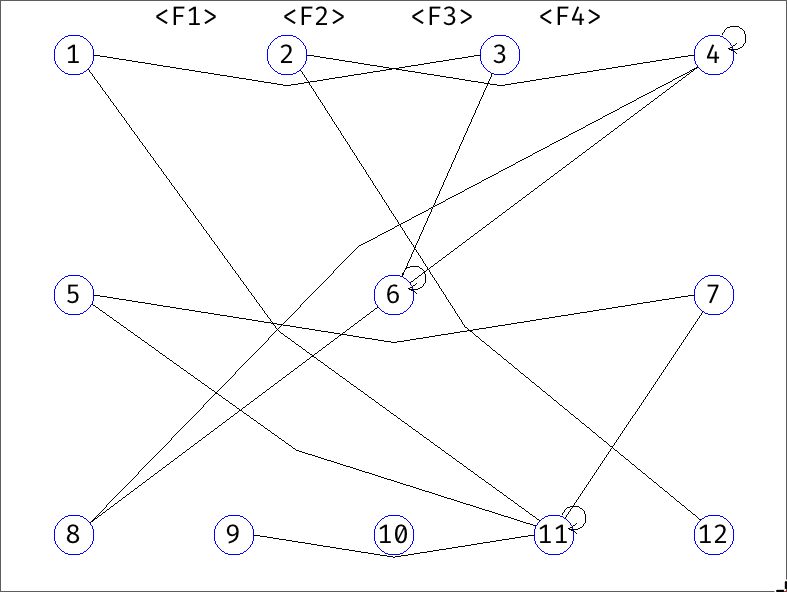
\includegraphics[width=0.5\linewidth]{undirected.png}
  \caption{Ненапрямлений граф}
\end{figure}
\begin{figure}[ht!]
  \center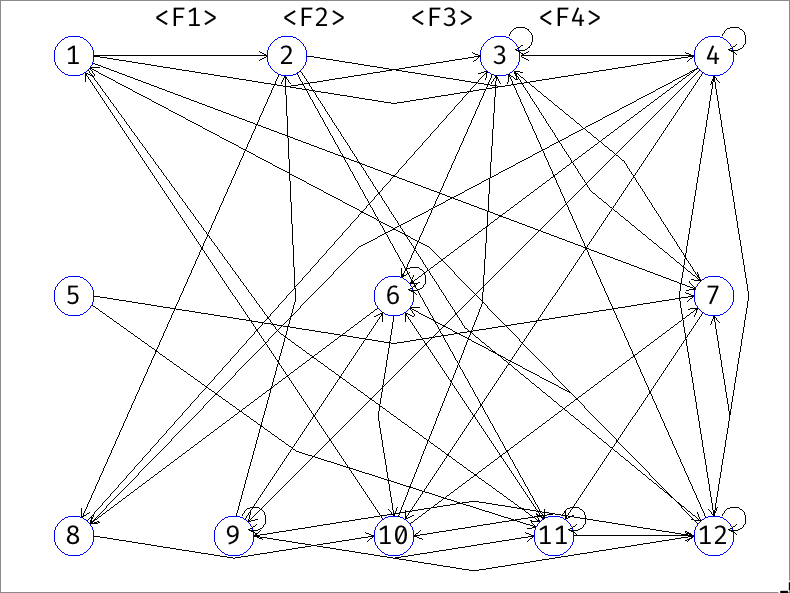
\includegraphics[width=0.5\linewidth]{modified.png}
  \caption{Модифікований граф}
\end{figure}
\begin{figure}[ht!]
  \center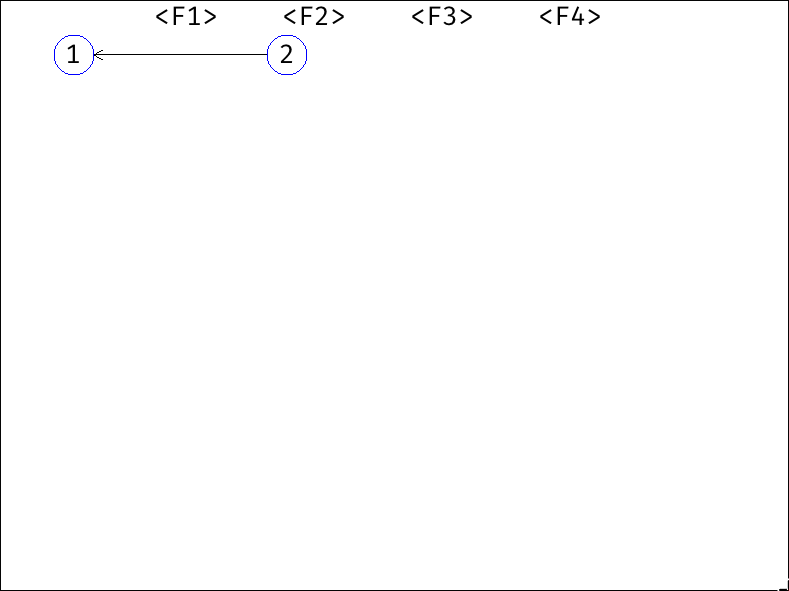
\includegraphics[width=0.5\linewidth]{condensed.png}
  \caption{Граф конденсації}
\end{figure}
\pagebreak

\conclusion%
Модифікував програму з ЛР №3, щоб вона працювала з графами динамічного розміру.
Застосував властивості графа для пошуку компонент сильної зв'язаності та побудови графа конденсації.

\end{document}

% vim: ts=2: sw=2
